\documentclass[10pt]{article}

%these two are needed for the tree drawings
\usepackage{graphicx,qtree}

%this package makes lists more compact
\usepackage{mdwlist}

%this is needed for \implies (and probably other stuff)
\usepackage{amsmath}
\usepackage{enumerate,amssymb,amsmath,amsthm} 
\usepackage[rightcaption]{sidecap}

%latexsym is needed for \Box
\usepackage{latexsym}

\usepackage{amssymb}
%This section is needed for the valuation brackets
\usepackage{tikz}
\usepackage[justification=centering]{caption}

\newcommand{\llbracket}{\
  \begin{tikzpicture}[scale=0.09,baseline=.3em]
  \draw (1.75,0) -- (0,0) -- (0,4) -- (1.75,4);
  \draw (1,0) -- (1,4);
  \end{tikzpicture}
  \
}
\newcommand{\rrbracket}{\
  \begin{tikzpicture}[scale=0.09,baseline=.3em]
  \draw (0,4) -- (1.75,4) -- (1.75,0) -- (0,0);
  \draw (.75,0) -- (.75,4);
  \end{tikzpicture}
  \
}

%This is me being a jerk about margins
\usepackage{geometry}
 \geometry{
 a4paper,
 total={210mm,297mm},
 left=20mm,
 right=20mm,
 top=10mm,
 bottom=20mm,
 }
 
\usepackage{listings}
\usepackage{color}

\definecolor{dkgreen}{rgb}{0,0.6,0}
\definecolor{gray}{rgb}{0.5,0.5,0.5}
\definecolor{mauve}{rgb}{0.58,0,0.82}

\lstset{frame=tb,
  language=Java,
  aboveskip=3mm,
  belowskip=3mm,
  showstringspaces=false,
  columns=flexible,
  basicstyle={\small\ttfamily},
  numbers=none,
  numberstyle=\tiny\color{gray},
  keywordstyle=\color{blue},
  commentstyle=\color{dkgreen},
  stringstyle=\color{mauve},
  breaklines=true,
  breakatwhitespace=true,
  tabsize=3
}

\begin{document}

%I hate the stock pound sign... so I fiddle with it here
\title{User Guide}
\author{Alister Maguire, Jared Paeschke, Garett Robert, Howard Lin}

\maketitle
\LARGE
\textbf{\textit{\underline{Setting Up Input Data}}}
\normalsize
\begin{enumerate}
\item[--] First step is to make sure you have a google drive account. You can create/verify it at \textbf{drive.google.com}.
\item[--] First add(copy) the templated form to your google drive by going to \\
\textbf{https://docs.google.com/forms/d/1TNLJhRqVsJgYPVE4l6FGnRVrklkV7Mnurv422yjAn3s/copy} \\
\begin{figure}[h]
\caption{You should see a website such as this.}
\centering

\includegraphics[width=0.75\textwidth]{pic1}
\end{figure}
\item[--] Go ahead and \textbf{click “Make a copy”} and you will be brought to your copy of the form. Once you see this form you should be able to see the format of it all.
\item[--] You can then distribute the form (so applicants can put in data) by \textbf{clicking the send button} in the top right corner.
\begin{figure}[h]
\caption{Click send}
\centering
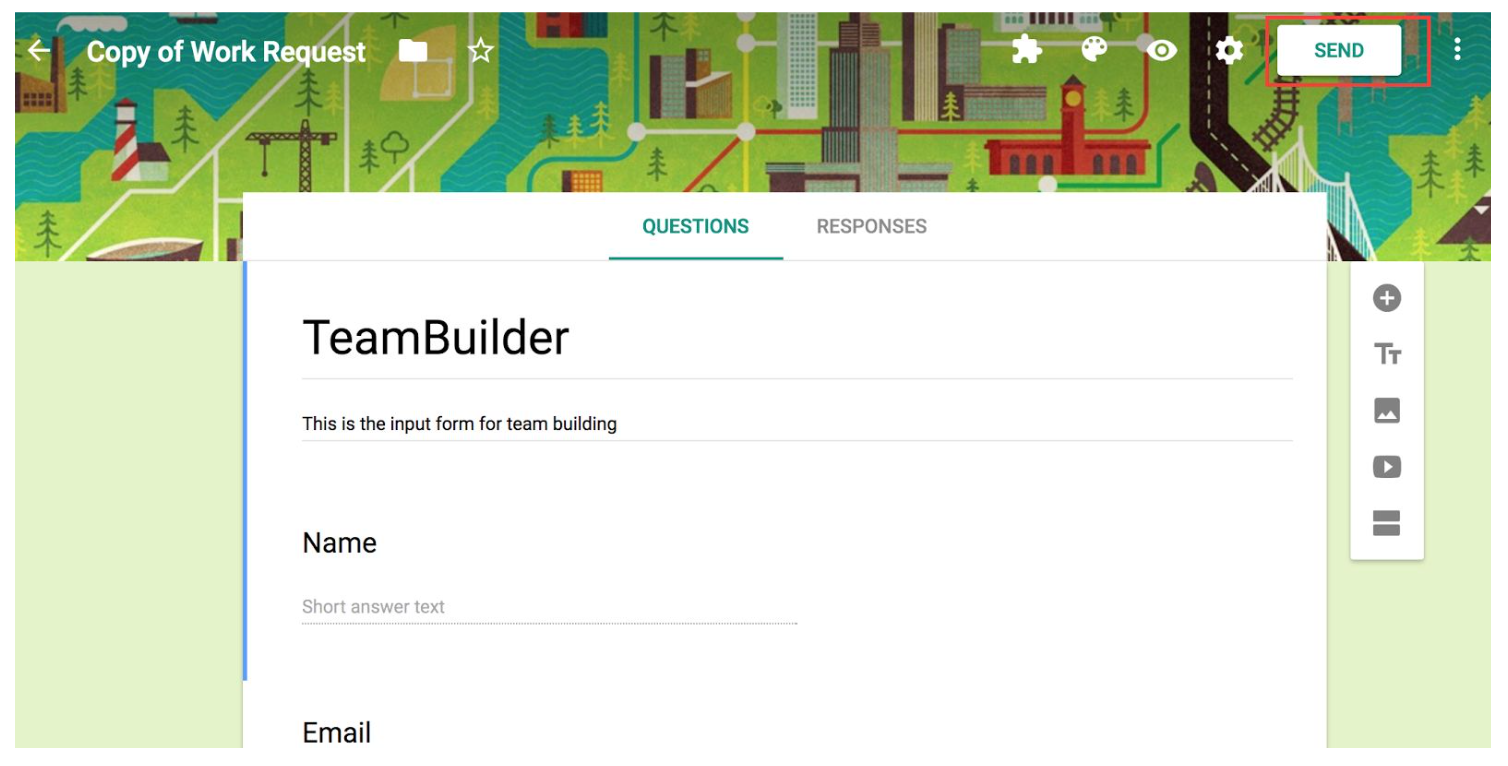
\includegraphics[width=0.8\textwidth]{pic2}
\end{figure}
\newpage
\item[--] \textbf{Click the link icon and shorten url, then copy.}  
\begin{figure}[h]
\caption{That link is the link that you want to distribute.}
\centering
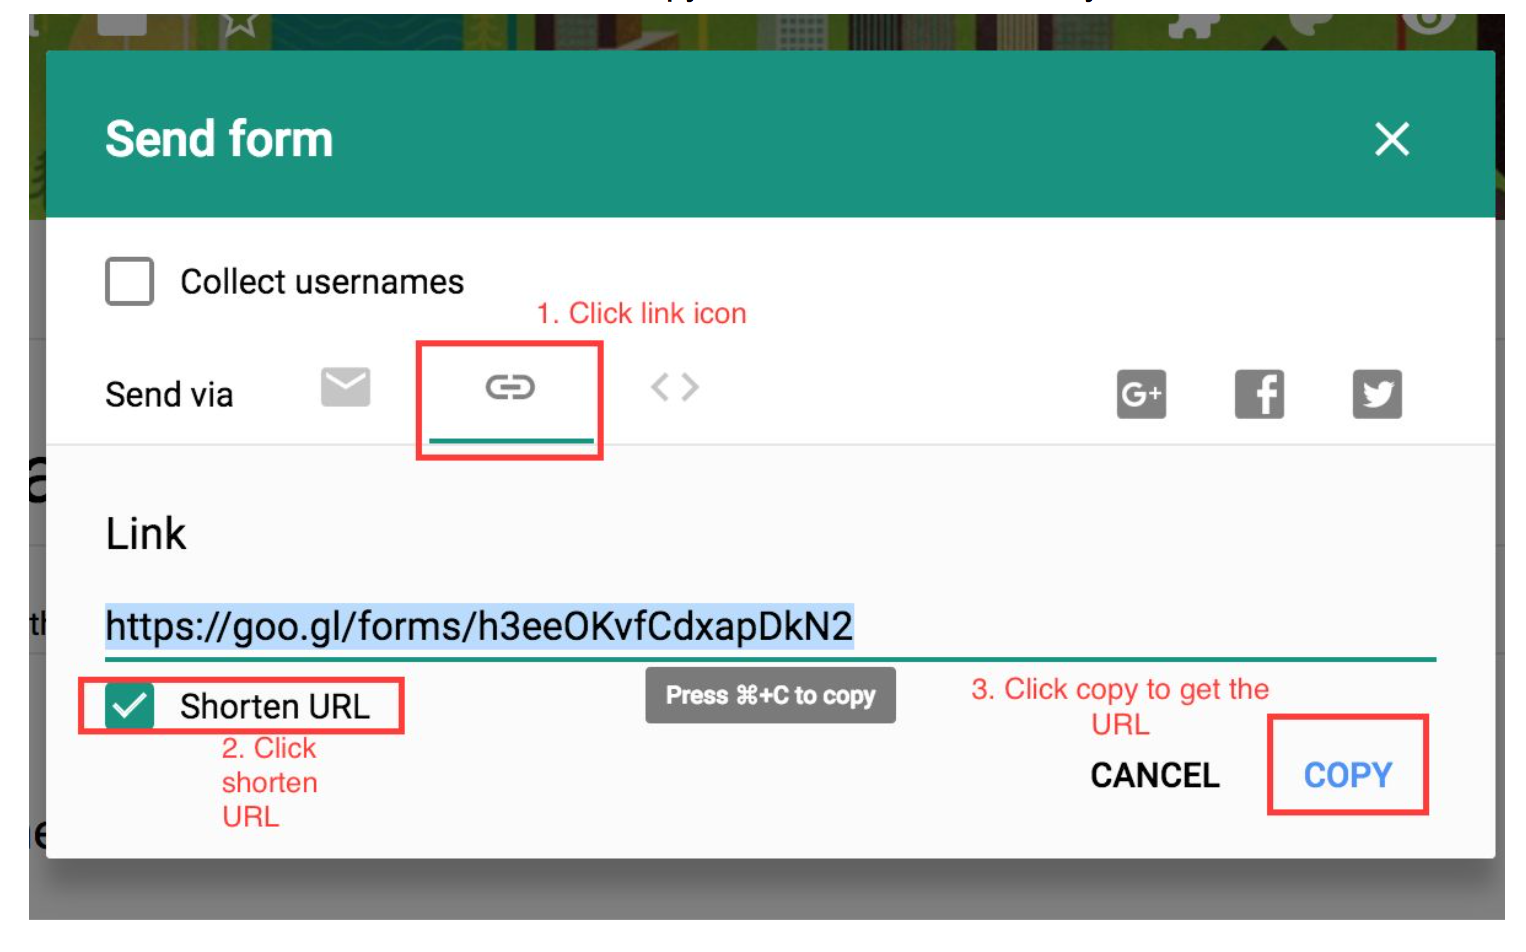
\includegraphics[width=0.5\textwidth]{pic3}
\end{figure}
\item[--] To check results/submissions, \textbf{click on the responses tab}
\begin{figure}[h]
\caption{Use this to keep track of submissions}
\centering
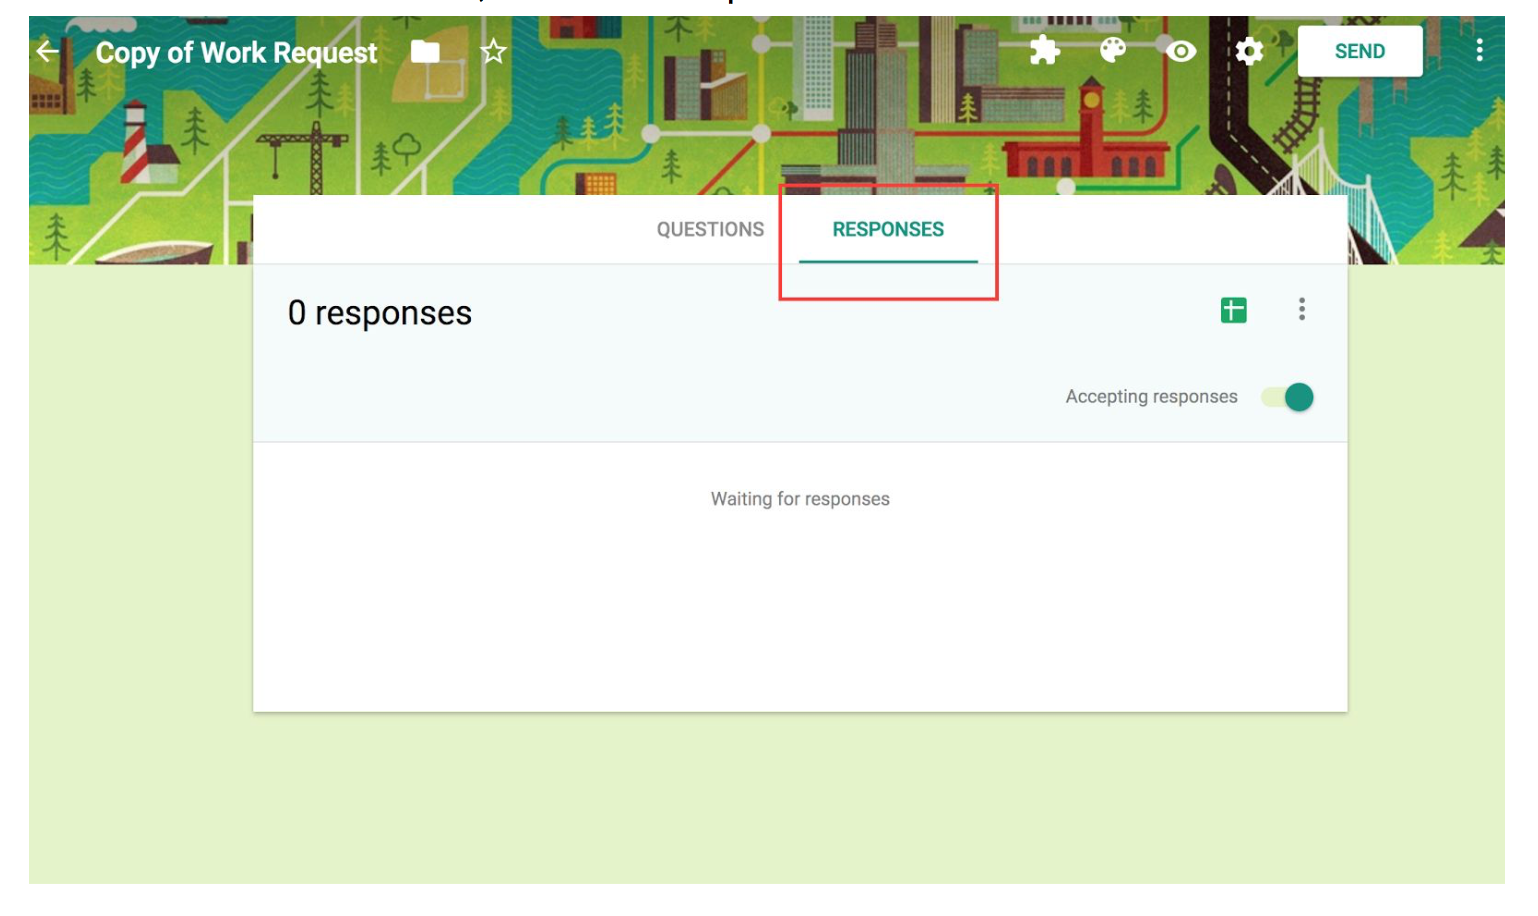
\includegraphics[width=0.5\textwidth]{pic4}
\end{figure}
\item[--] Once submissions are in, \textbf{click the green box in responses}
\begin{figure}[h]
\caption{After data is collected, we start creating the CSV}
\centering
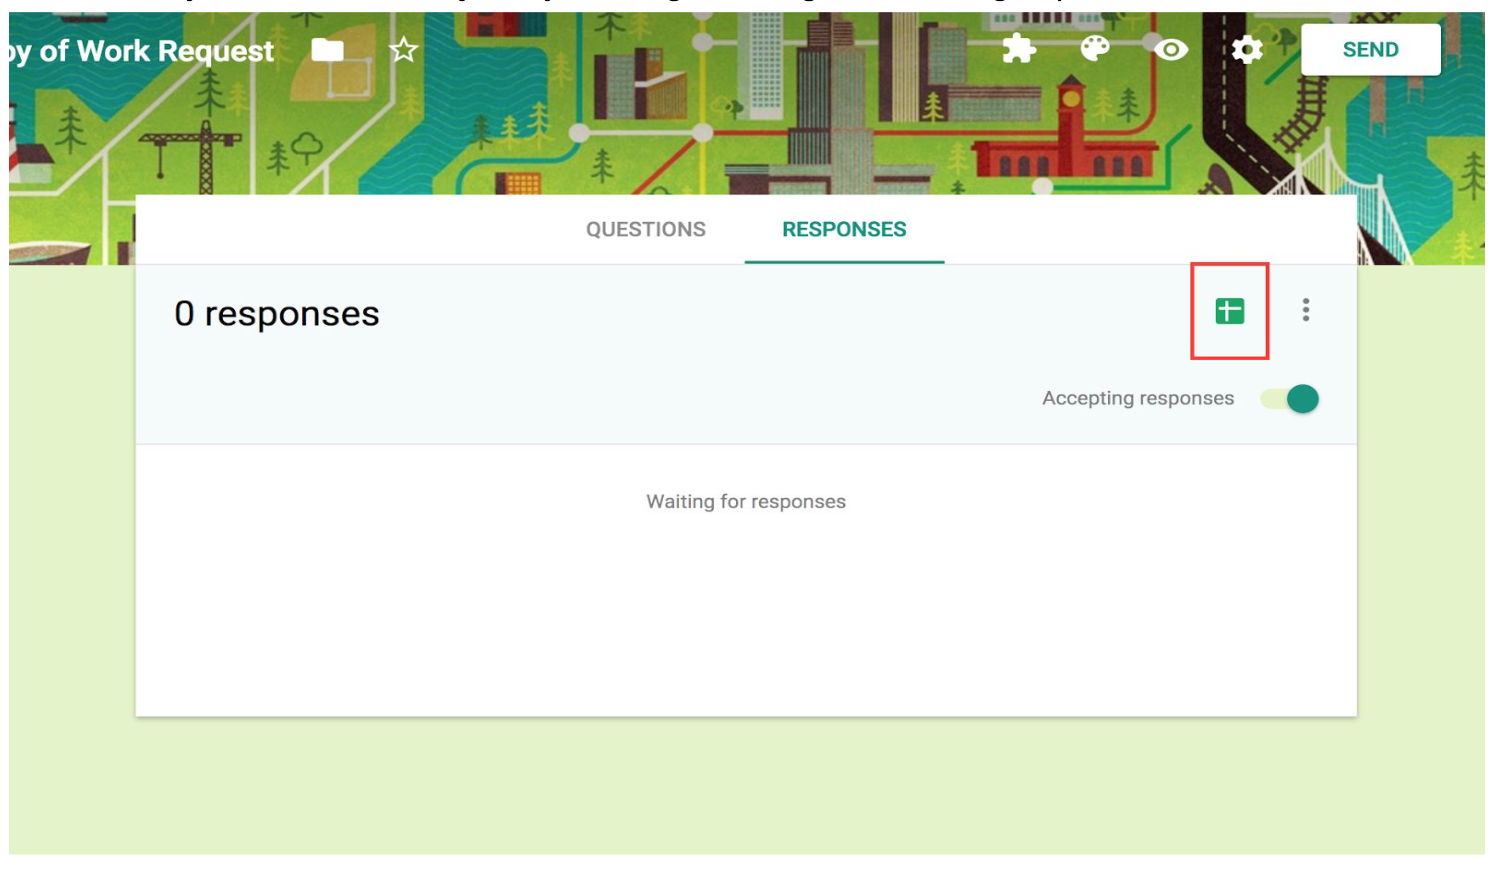
\includegraphics[width=0.6\textwidth]{pic5}
\end{figure}\\
\textit{Note} that if any responses come in later after creating the excel sheet, they will be automatically added to it, you can access it just by clicking on the green icon again.
\newpage
\item[--] Once clicked it will ask you to create an excel sheet or select an existing excel sheet. \textbf{Click Create and Change the name if you desire, then click create.}
\begin{figure}[h]
\caption{This will create an excel sheet}
\centering
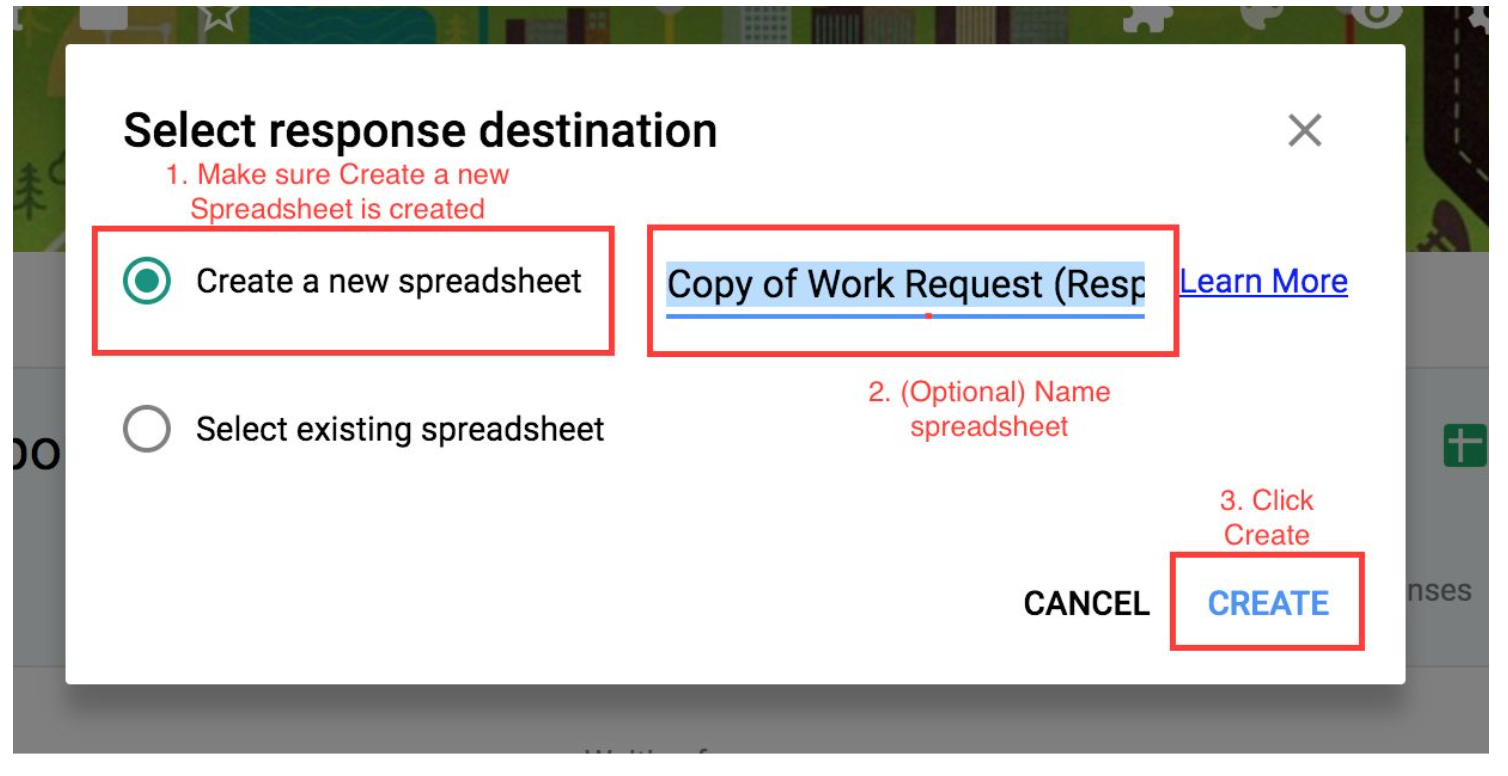
\includegraphics[width=0.45\textwidth]{pic6}
\end{figure}
\item[--] After clicking create it will bring you to a spreadsheet with all your data. We want to \textbf{export} this as an \textbf{\textit{csv file}}. To do this, go to \textbf{“file”} then \textbf{“Download as”} then select \textbf{“Comma-separated values”}
\begin{figure}[h]
\caption{We export to a CSV file}
\centering
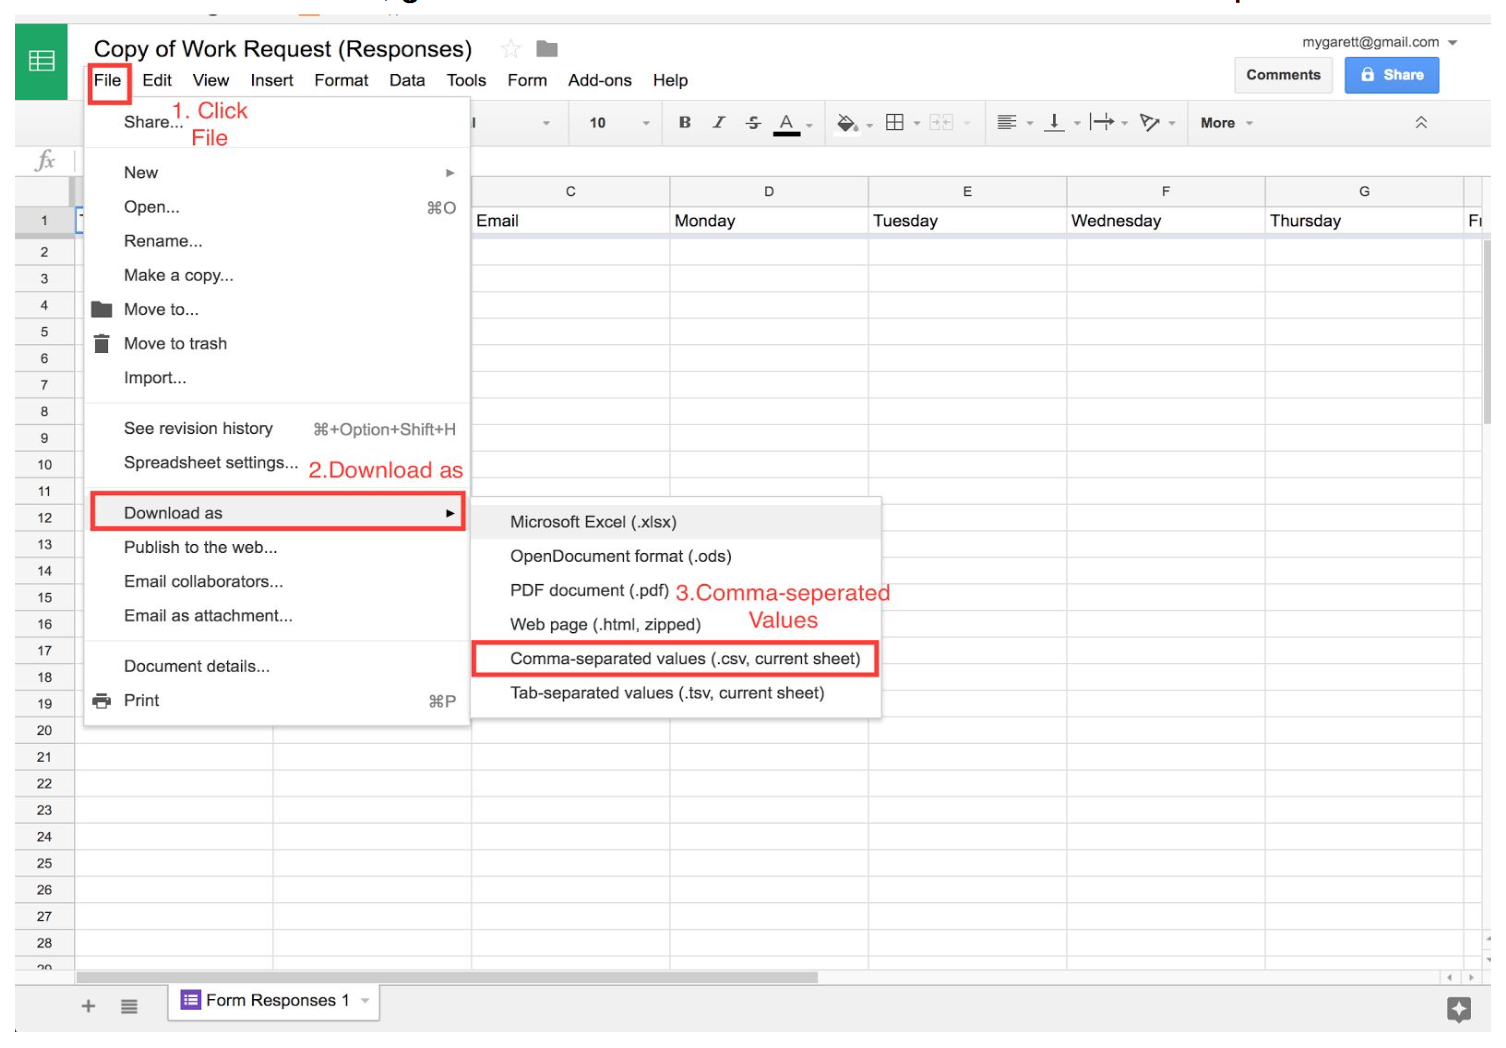
\includegraphics[width=0.7\textwidth]{pic7}
\end{figure}
\item[--] Before we continue, you need to create a \textbf{\textit{txt file}} with a student roster (just with all of their names) (below for example). New line separated, with last name first, comma, space, and first name
\begin{figure}[h]
\caption{Creating the team roster}
\centering
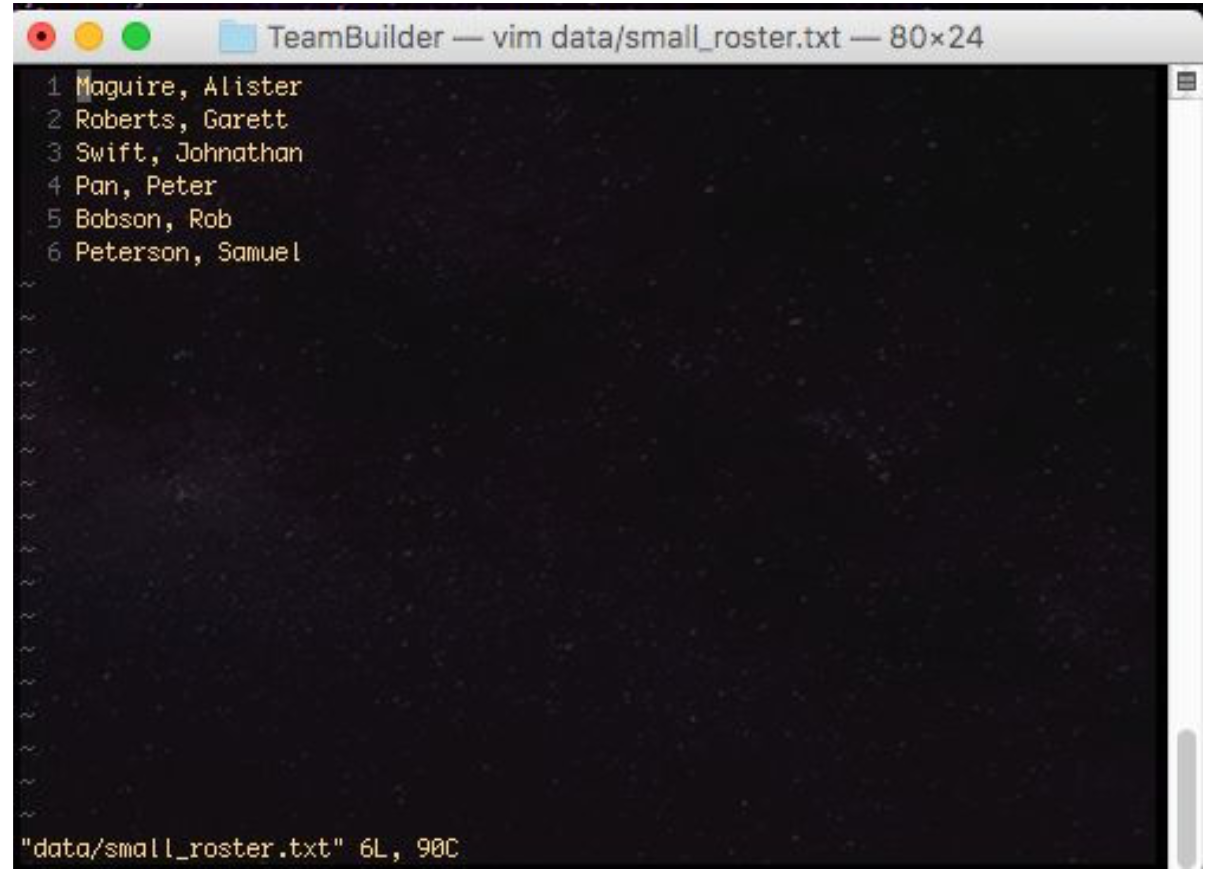
\includegraphics[width=0.35\textwidth]{pic8}
\end{figure}\\
\textbf{Congratulations! You have finished setting up the desired input data. Save those files and proceed to running the GUI}
\newpage
\maketitle
\LARGE
\textbf{\textit{\underline{Running the GUI}}}
\normalsize
\item[--] In the directory, \textbf{double click on Run} to start the GUI. 
\begin{figure}[h]
\caption{Run will run the GUI}
\centering
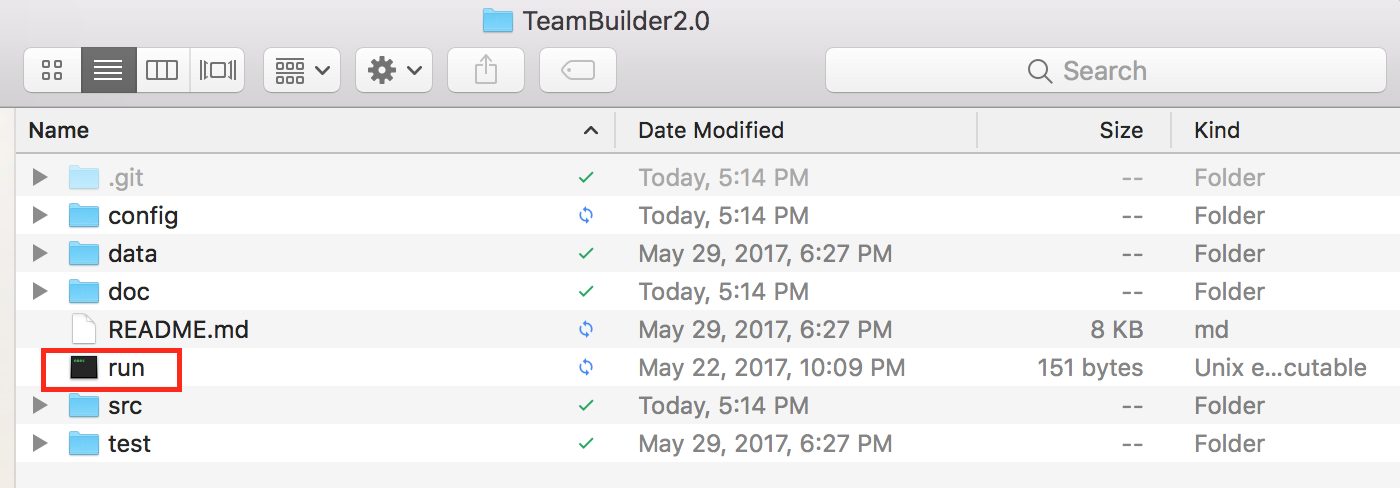
\includegraphics[width=0.35\textwidth]{pic9}
\end{figure}\\
\textbf{\textit{NOTE}} if Run is not working correctly, you can also start the GUI by opening a terminal and running\\
\begin{lstlisting}
$ python3 src/gui.py
\end{lstlisting}
In the directory\\
\item[--] You should then be greeted by the following screen. \textbf{Click on \textit{Browse}} to start inputting data for all of the fields. 
\begin{figure}[h]
\caption{This is the setup screen of the GUI}
\centering
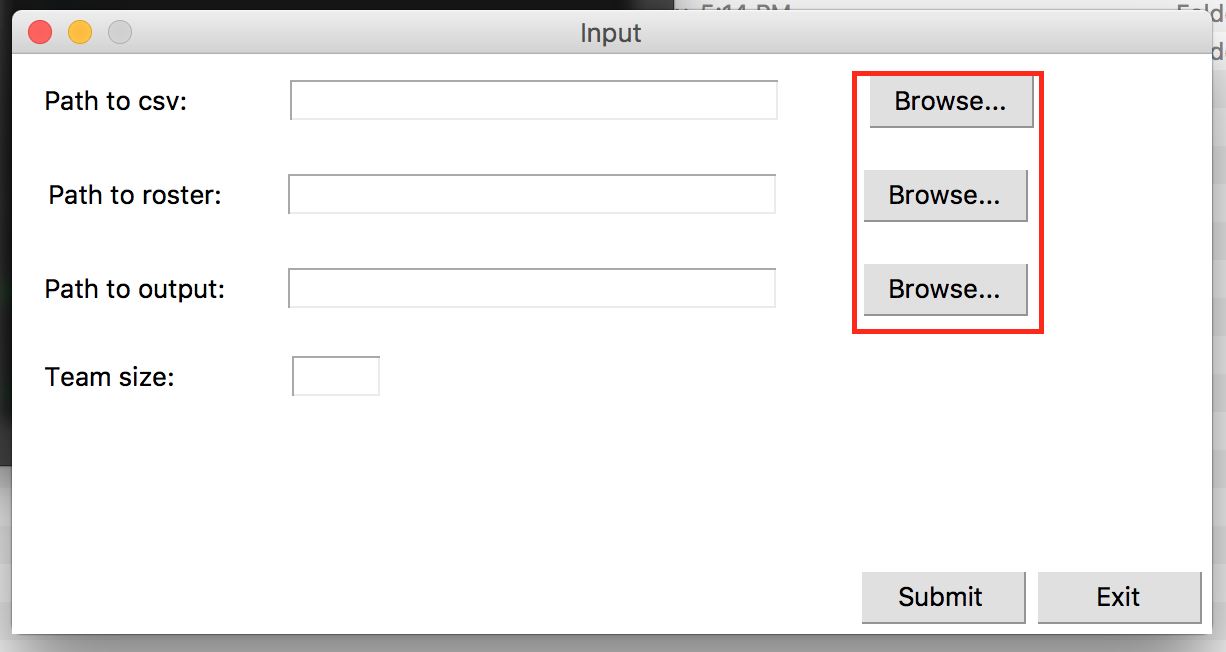
\includegraphics[width=0.6\textwidth]{pic10}
\end{figure}\\
\item[--] For each fields, use the file finder to \textbf{find your data files}, and then \textbf{click \textit{open}}. For Path to output, just find a directory where you want to save your outputs or a file you want to save it to.
\begin{figure}[h]
\caption{Input screen}
\centering
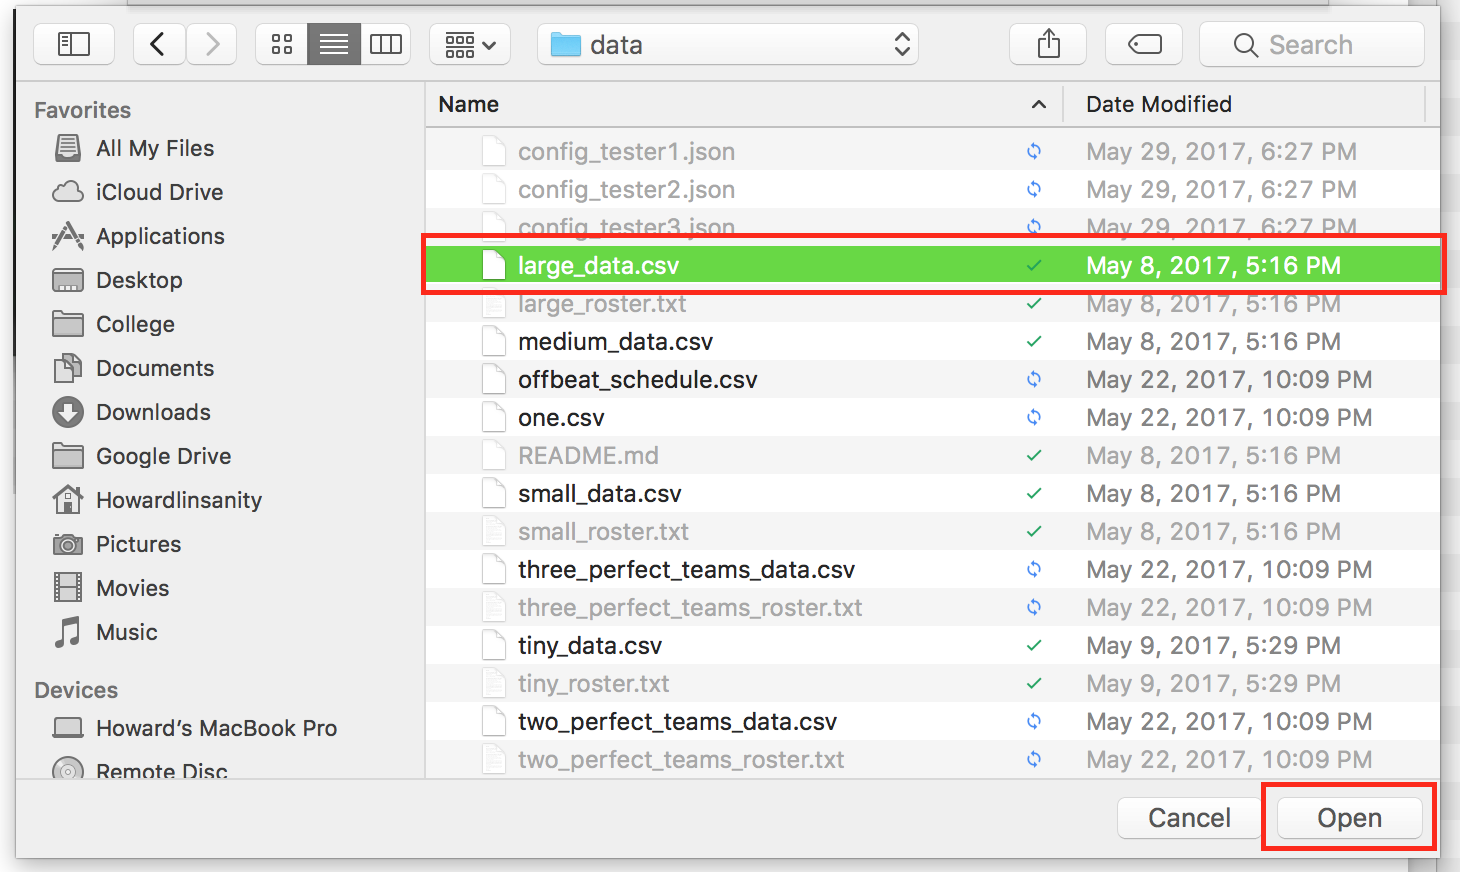
\includegraphics[width=0.6\textwidth]{pic11}
\end{figure}\\
\newpage
\item[--] After you put in all files and the team size, \textbf{click on \textit{Submit}}
\begin{figure}[h]
\caption{Let's start the algorithm!}
\centering
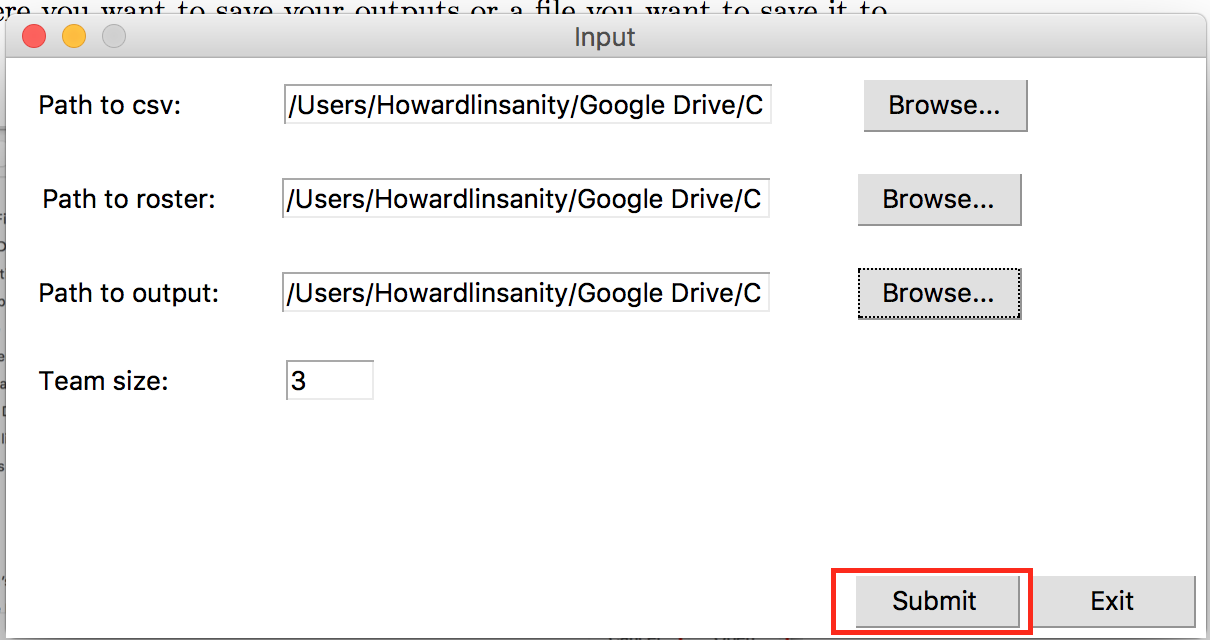
\includegraphics[width=0.6\textwidth]{pic12}
\end{figure}\\
\item[--] After running the algorithm, you should then be greeted by the results screen, which displays the teams, their scores, and a few options if you choose to twiddle with the results.
\begin{figure}[h]
\caption{Results screen}
\centering
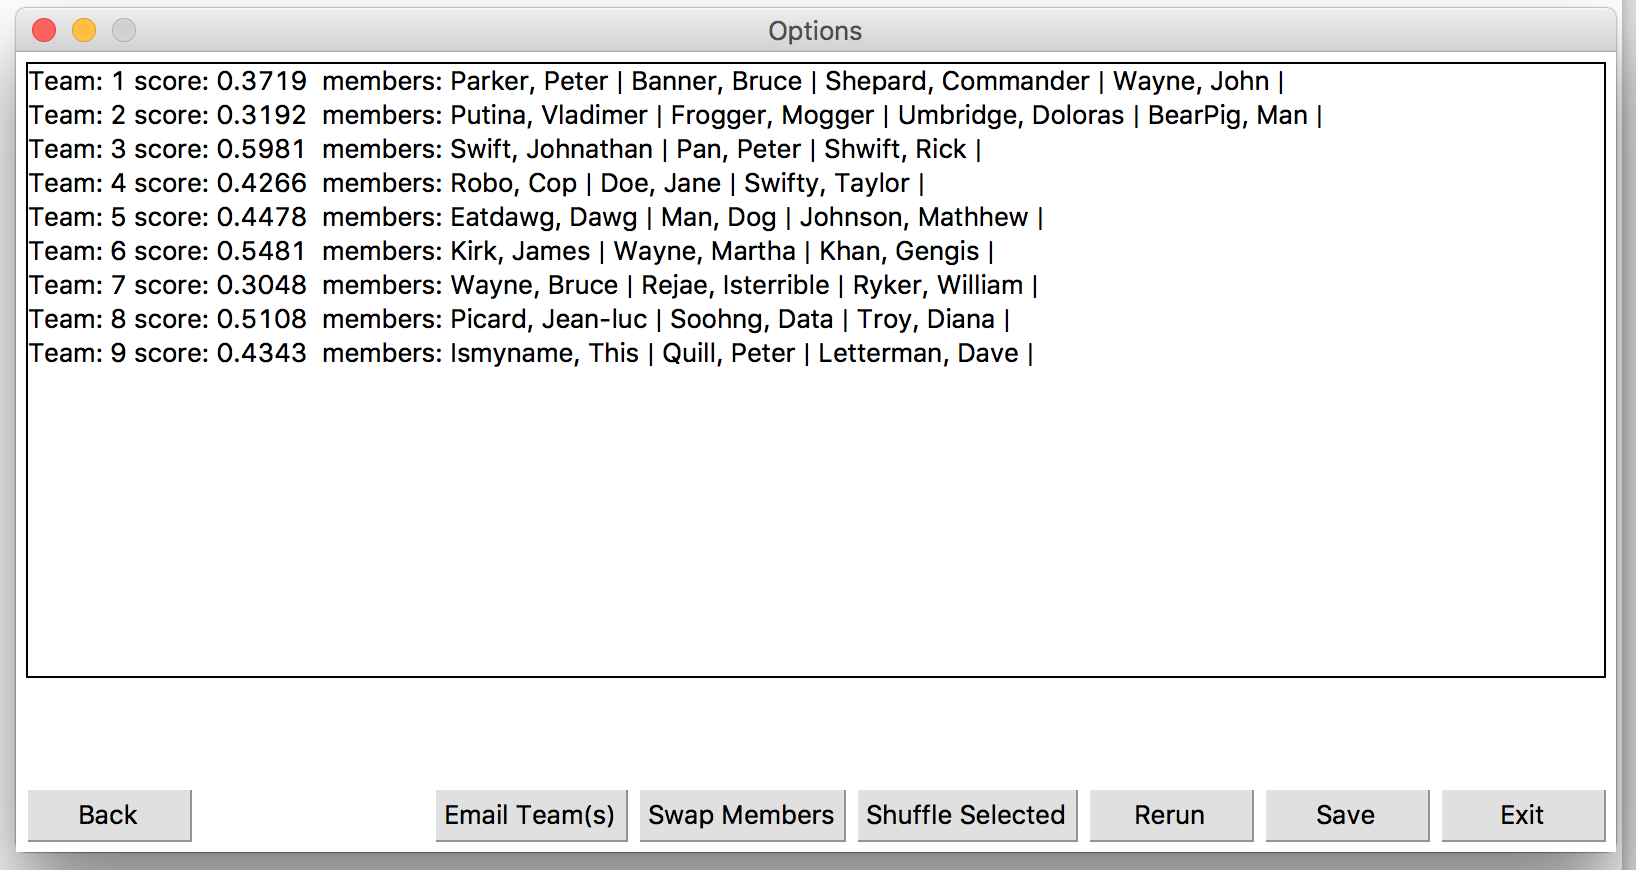
\includegraphics[width=0.6\textwidth]{pic13}
\end{figure}\\
\newline
\maketitle
\LARGE
\textbf{\textit{\underline{Options and Features}}}
\normalsize
\newline
\newline
Now that you have the teams assembled and scored, you now have these tools and options to modify the team selection.
\item[--] To \textbf{inspect} the individual teams, \textbf{double click} a team to open up the team inspection teams
\begin{figure}[h]
\caption{Note: If you double click in a way such that the last click "un-selects" a team, \newline you may be asked to try again}
\centering
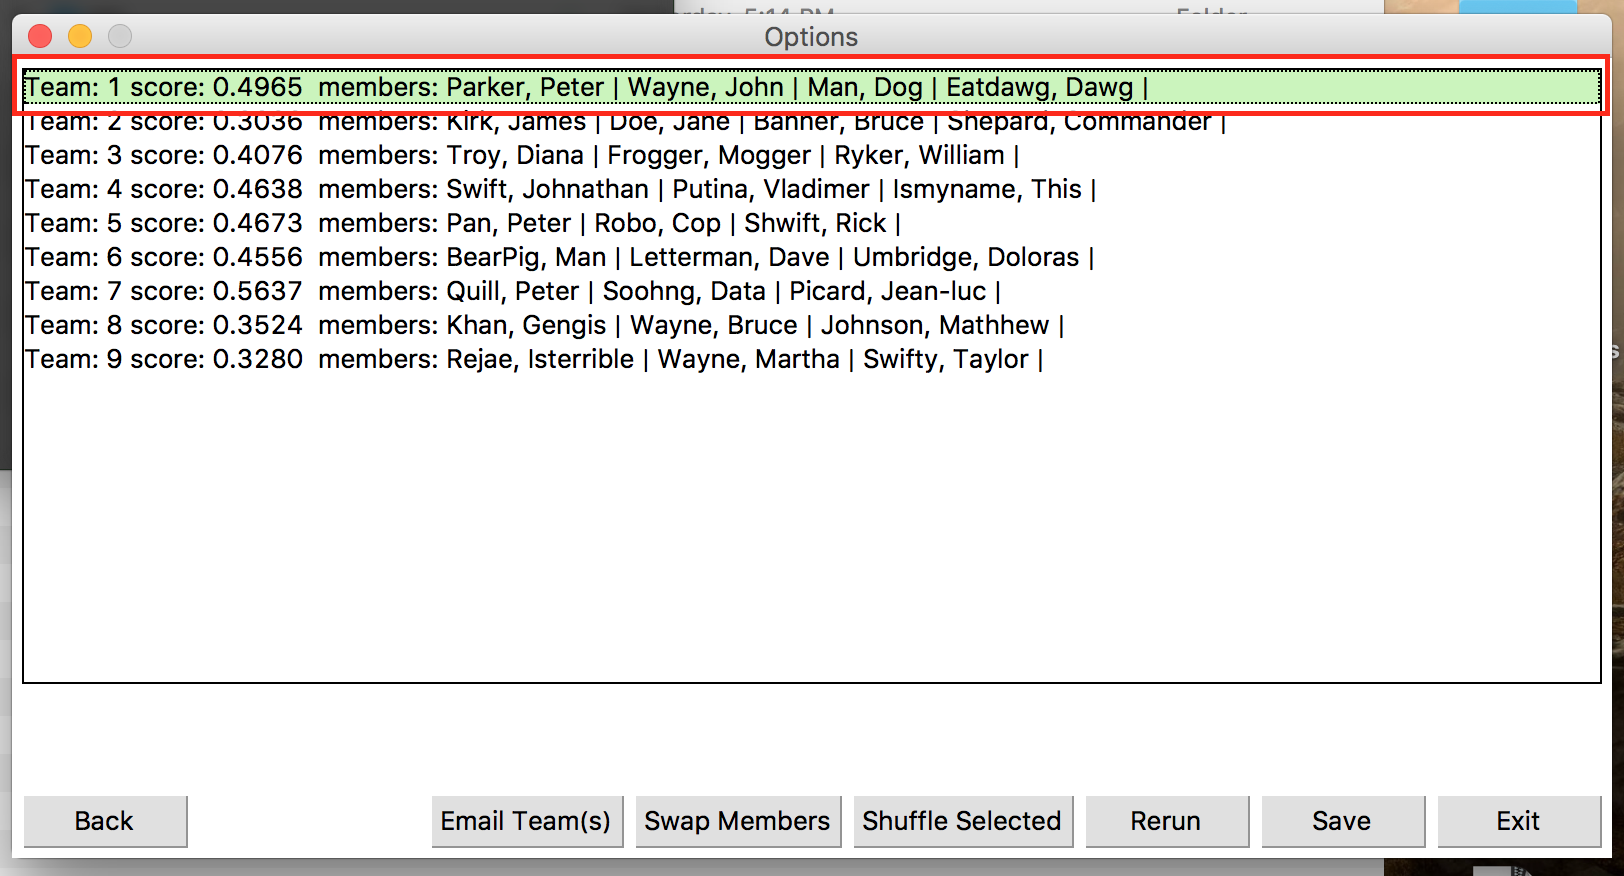
\includegraphics[width=0.6\textwidth]{pic14}
\end{figure}\\
\newpage
The following information may be useful in swapping out individual members, which we will get to next
\begin{figure}[h]
\caption{To go back to the main screen, hit close}
\centering
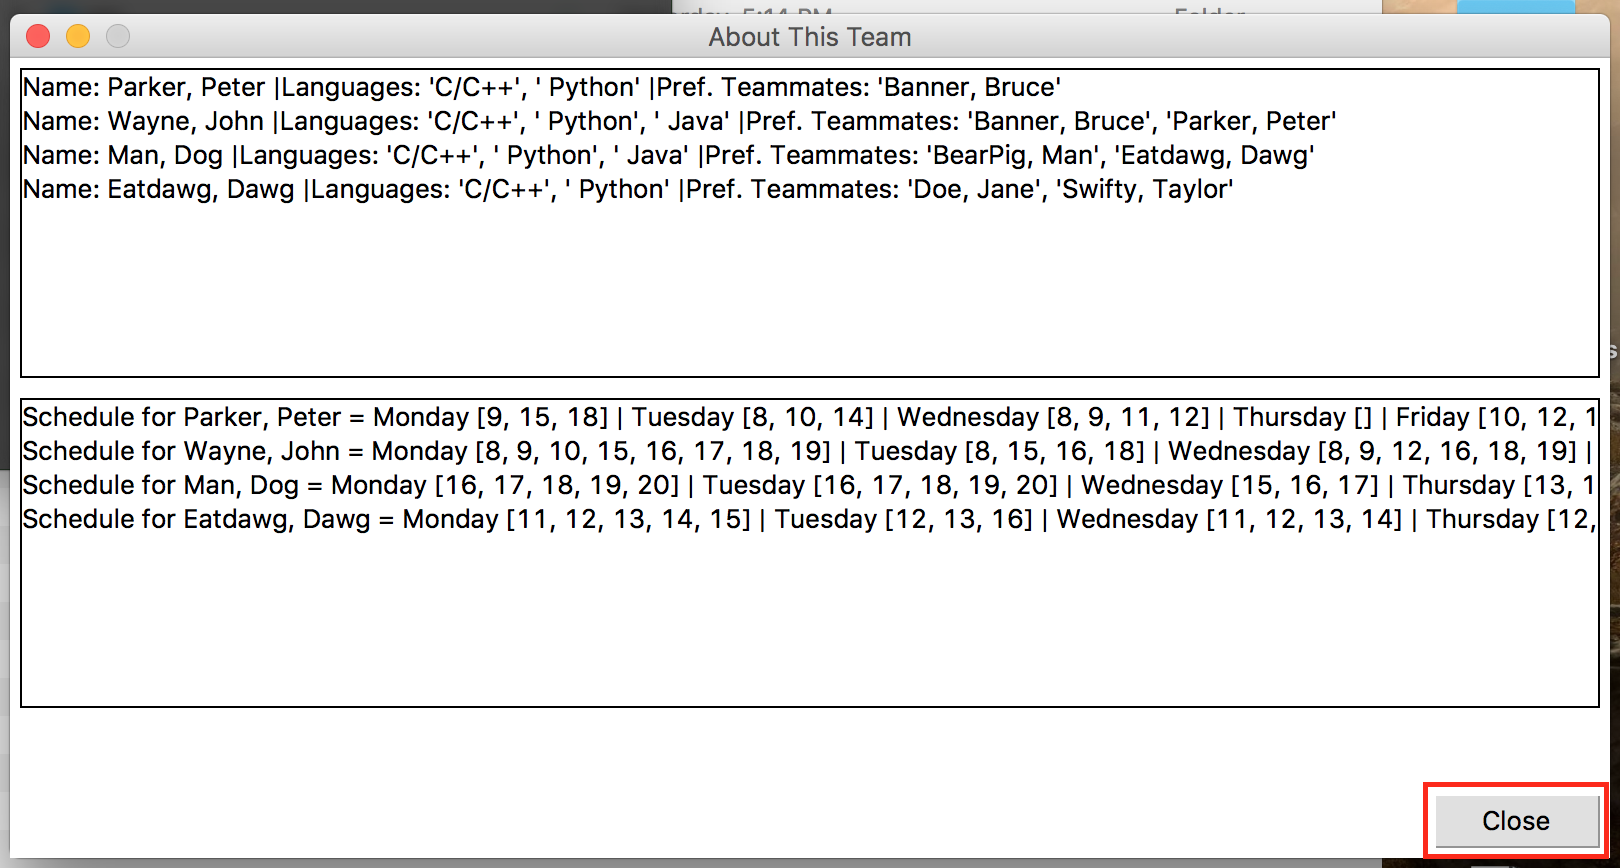
\includegraphics[width=0.6\textwidth]{pic15}
\end{figure}\\
\item[--] To swap individual members between two teams, \textbf{click on two teams} and then click on \textbf{\textit{Swap Members}}
\begin{figure}[h]
\caption{Select exactly 2 teams before clicking Swap Members}
\centering
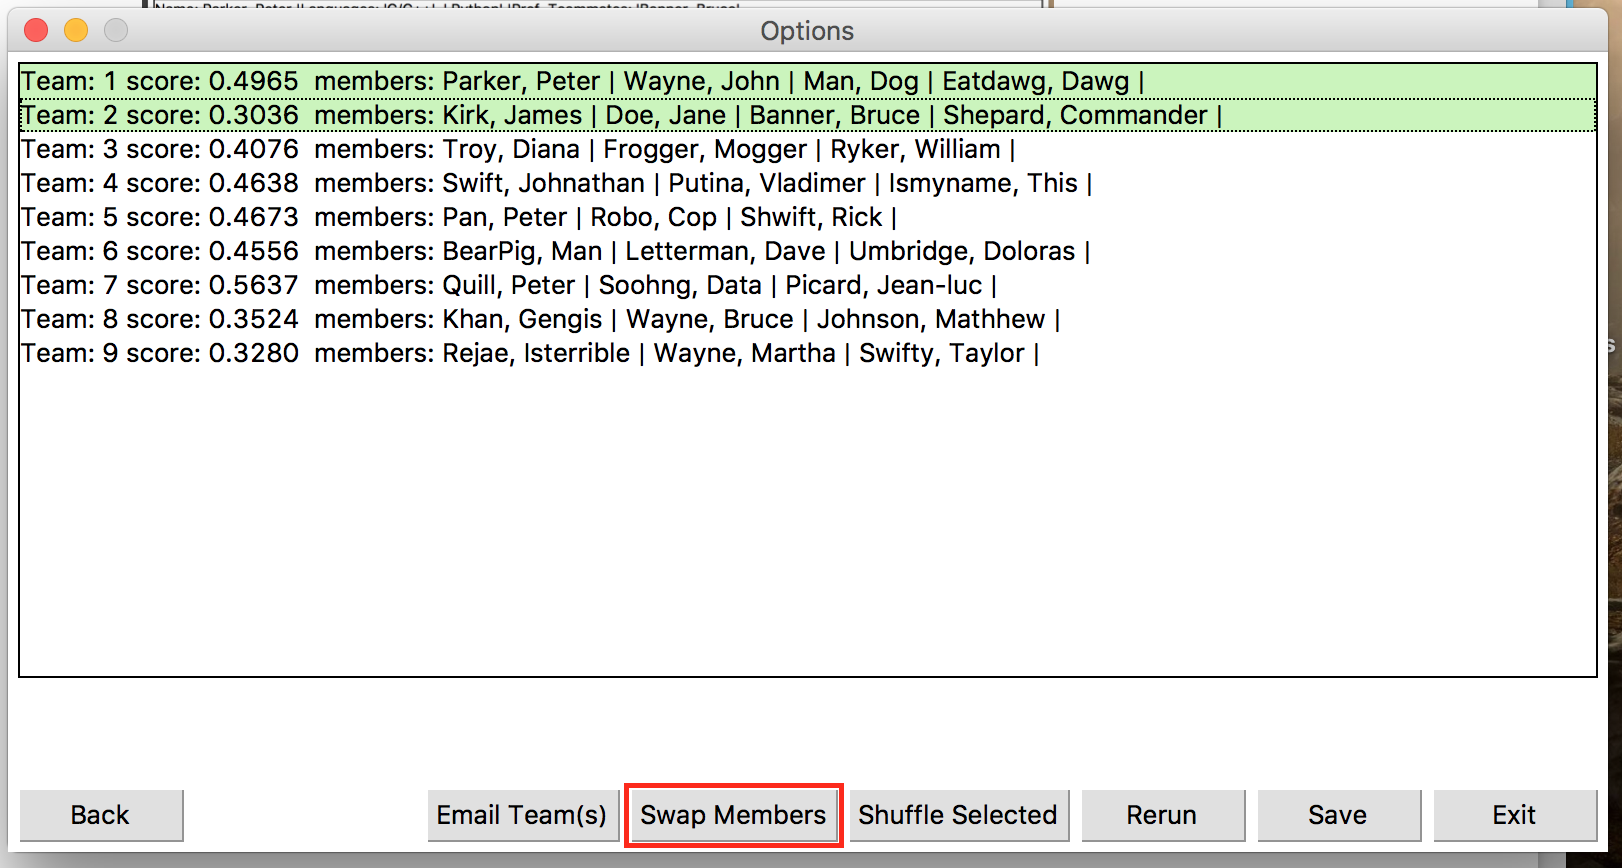
\includegraphics[width=0.6\textwidth]{pic16}
\end{figure}\\
You will then be greeted by the following screen, and to swap members, \textbf{select an individual}, and then \textbf{click on \textit{Swap Team}}
\begin{figure}[h]
\caption{When you are done, click on \textbf{\textit{Back}} to return to Options}
\centering
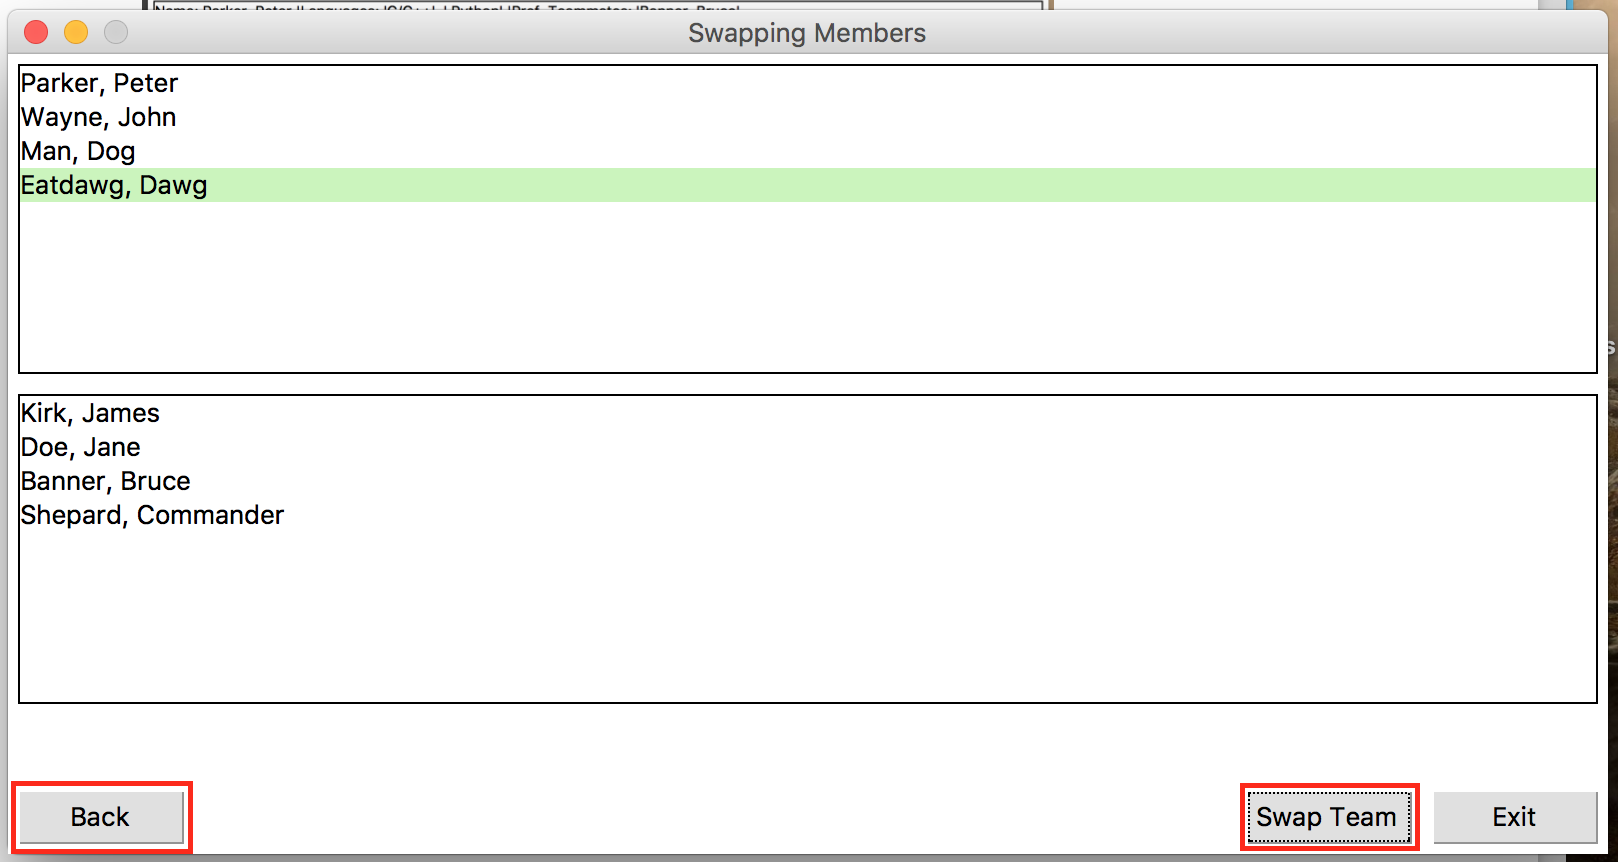
\includegraphics[width=0.6\textwidth]{pic17}
\end{figure}\\
\newpage
\item[--] To randomly reshuffle certain teams (switching members among a set of teams), \textbf{select the teams} you would like to reshuffle, and then \textbf{click on \textit{Shuffle Selected}}
\begin{figure}[h]
\caption{Select exactly 2 teams before clicking Swap Members}
\centering
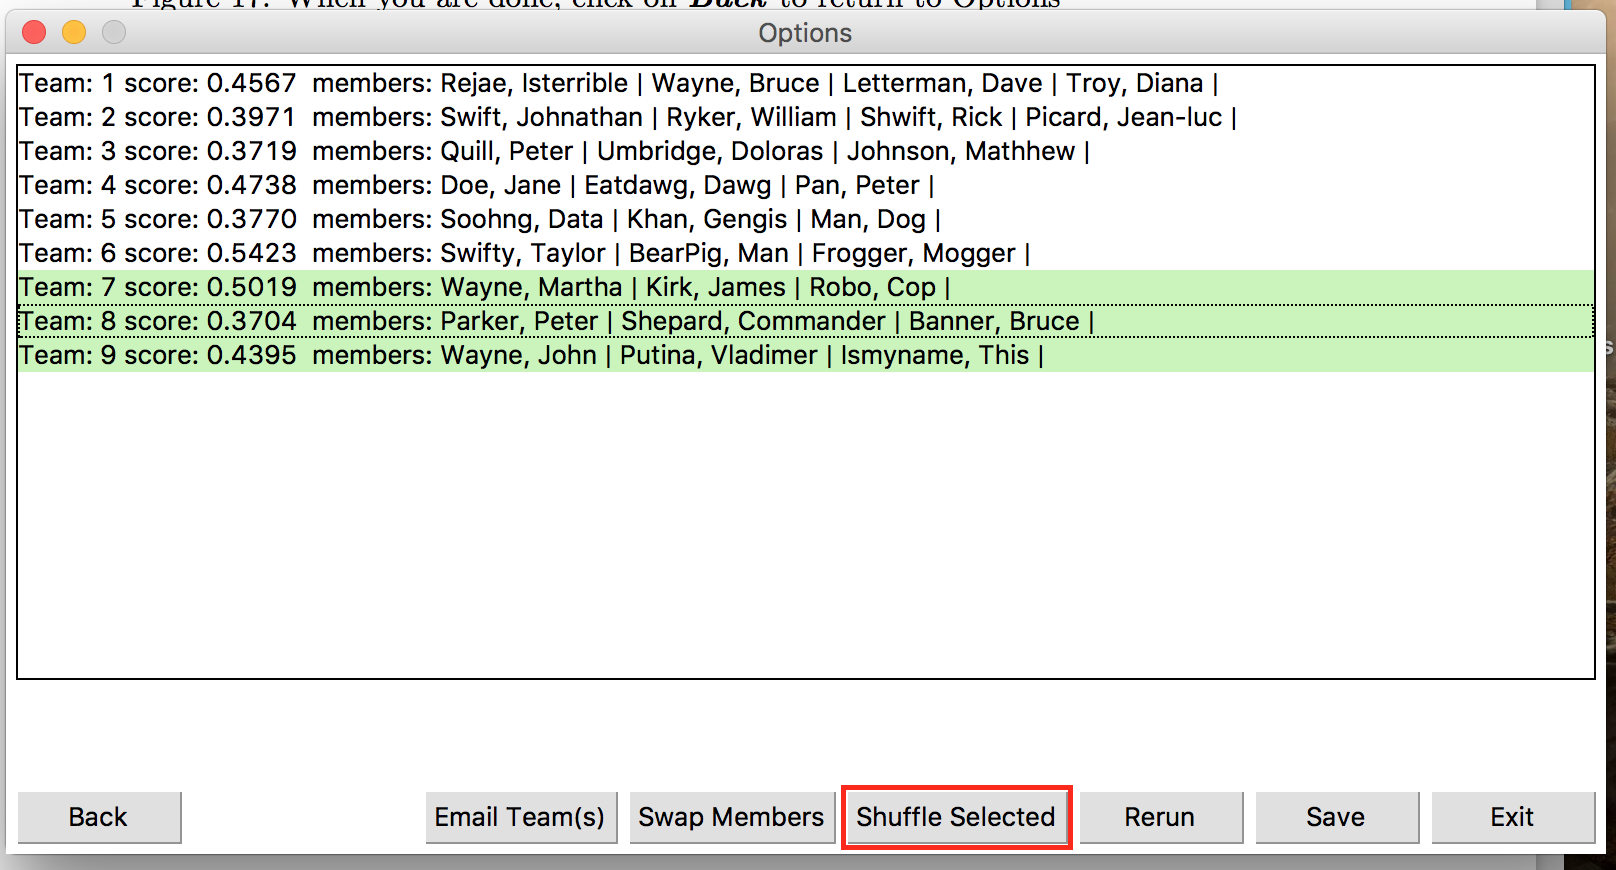
\includegraphics[width=0.6\textwidth]{pic18}
\end{figure}\\
\item[--] If you would like to rerun the whole algorithm and remake the groups from scratch, \textbf{click on \textit{Rerun}}
\begin{figure}[h]
\caption{Rerun}
\centering
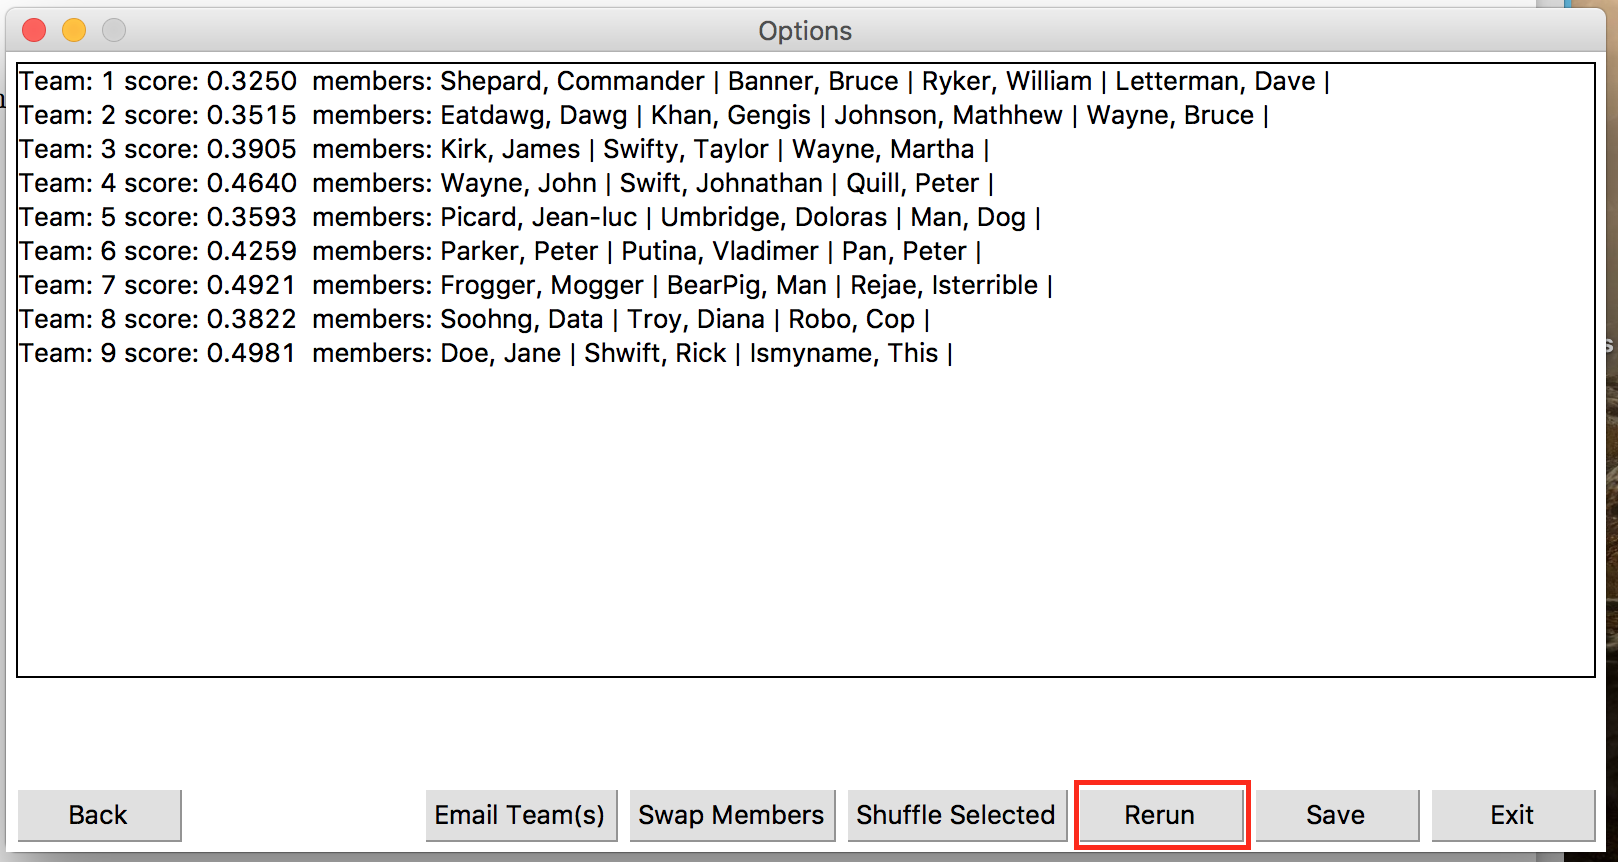
\includegraphics[width=0.6\textwidth]{pic19}
\end{figure}\\
\item[--] When you are done tweaking groups, you can save the results into a file by \textbf{clicking on \textit{Save}}. 
\begin{figure}[h]
\caption{The output file will be saved into the output destination selected during setup}
\centering
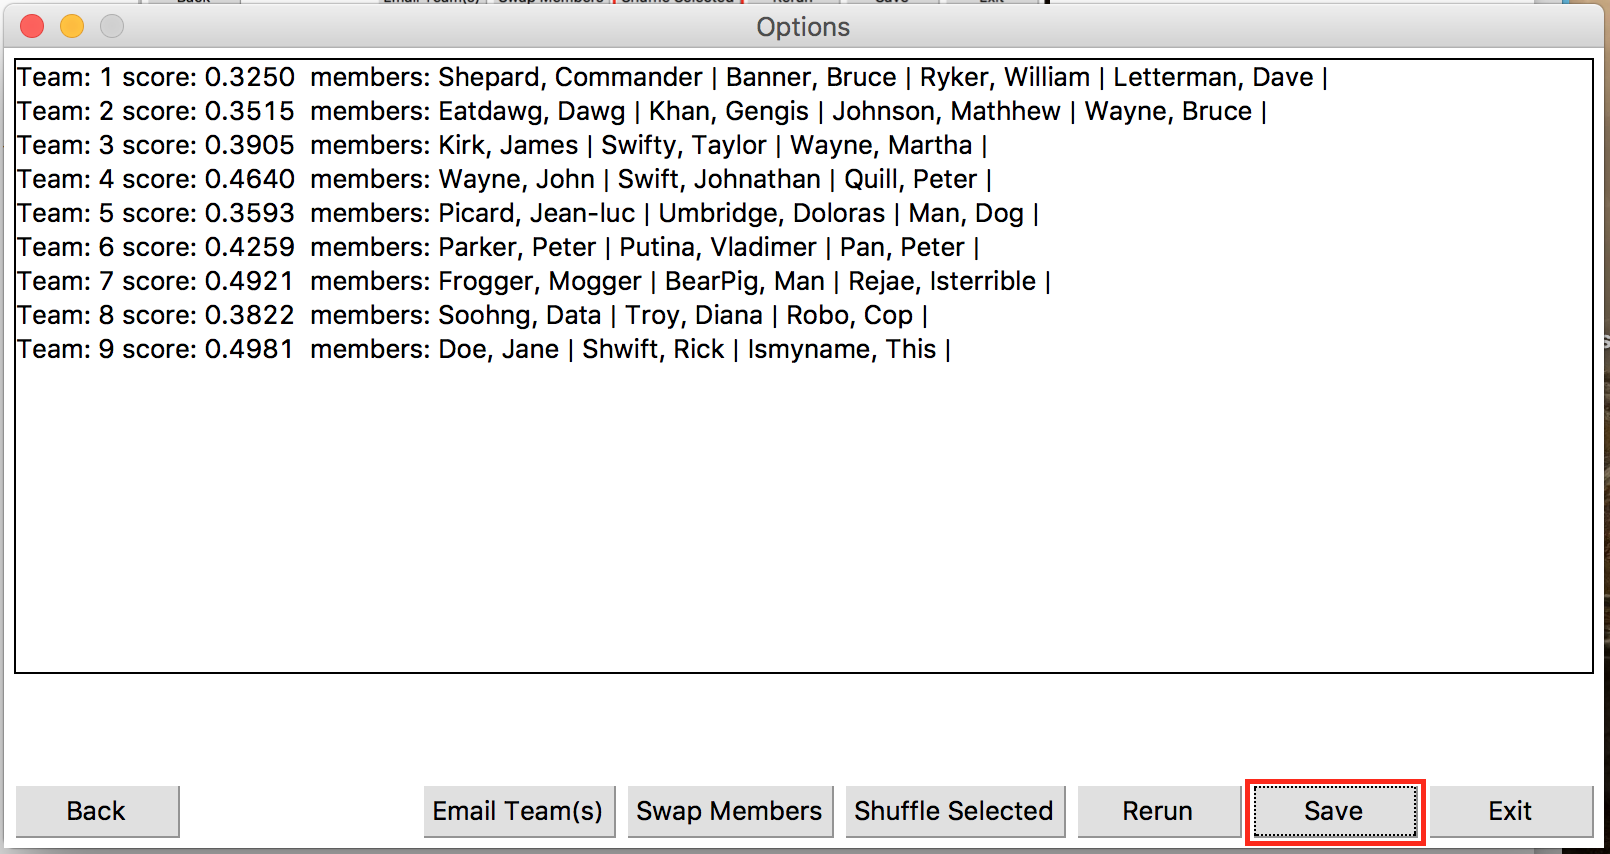
\includegraphics[width=0.6\textwidth]{pic20}
\end{figure}\\
Congratulations! You have now formed your group, but if you wish to inform and email your teams, do not hit exit yet. 
\newpage
\maketitle
\LARGE
\textbf{\textit{\underline{Informing Teams}}}
\normalsize
\newline
\newline
After you have created teams it is natural that you will want notify those individuals on the team who their new teammates are. In this project we have included a simple text only emailer to handle this for you. You can do this through cmdline or through the GUI that has been created. Regardless of how you wish to use the emailer you must first configure the email settings in the config directory.\\
\newline
\large
\textbf{Configure}
\normalsize
\newline
To configure the emailer find the config.json file located within the config directory. Open this and locate the email settings. 
\begin{figure}[h]
\caption{The following is an explanation of each setting}
\centering
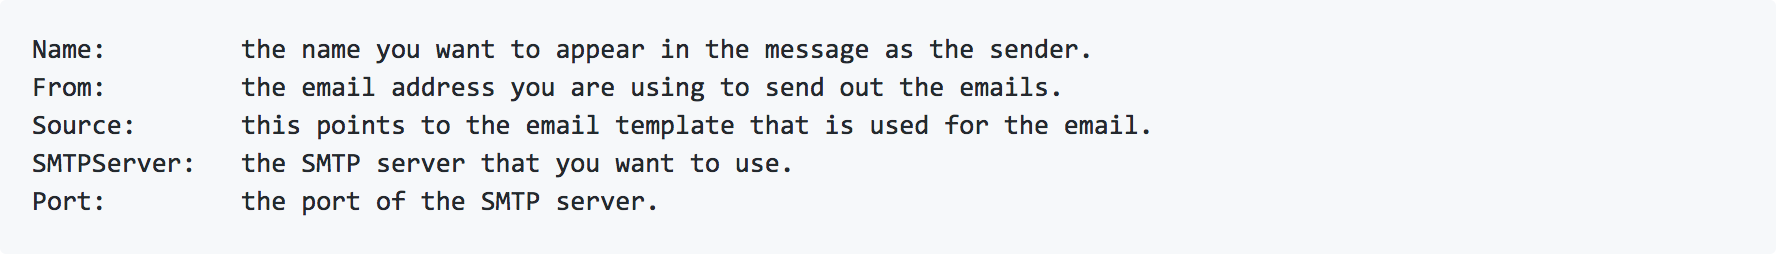
\includegraphics[width=0.9\textwidth]{pic21}
\end{figure}\\
\newline
\large
\textbf{Command Line Usage}
\normalsize
\newline
To email the created teams you will want to first run the program to generate teams. When you do this you will have a text file of output. Using this output is how you will email the teams out. From the main directory of the repository run the command
\begin{lstlisting}
$ python3 src/inform.py ../output.txt
\end{lstlisting}
In the above hypothetical the output.txt is located in the main directory. The inform.py will look for the file relative to its location on the file system. This is why in the example above the argument points to the parent directory.
\newline
\newline
You will next see a prompt requesting your login/password for the SMTP server. After supplying them the emails will be sent. The format of the email is determined by the email template. Details on changing this is located below.\\
\newline
\large
\textbf{GUI Usage}
\normalsize
\newline
To access the emailer within the GUI version of the program, you start it as normal. Once you have generated the teams and adjusted them a you want, to email the teams first select all the teams that you want to email. Next locate the email button at the lower edge of the window. Hit it and then a new window will appear asking for the login/passsword for the SMTP server specified in the config settings. After entering this info hit send and the emails will be sent. 
\begin{figure}[h]
\caption{Select the teams that you want to notify}
\centering
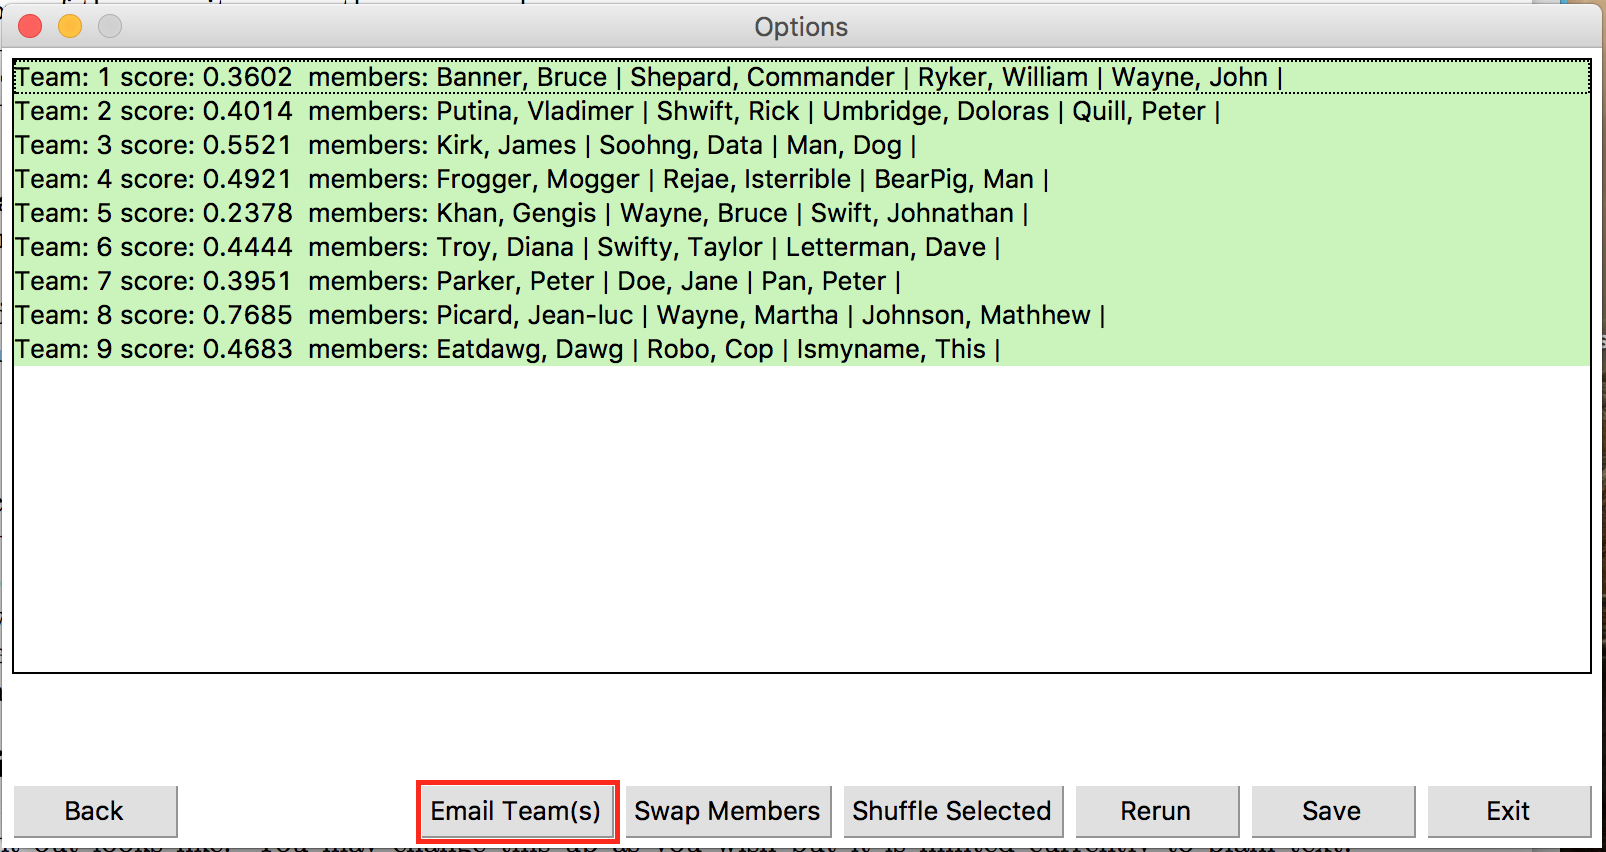
\includegraphics[width=0.6\textwidth]{pic22}
\end{figure}\\
\newpage
\begin{figure}[h]
\caption{Then input your credentials and then hit Submit}
\centering
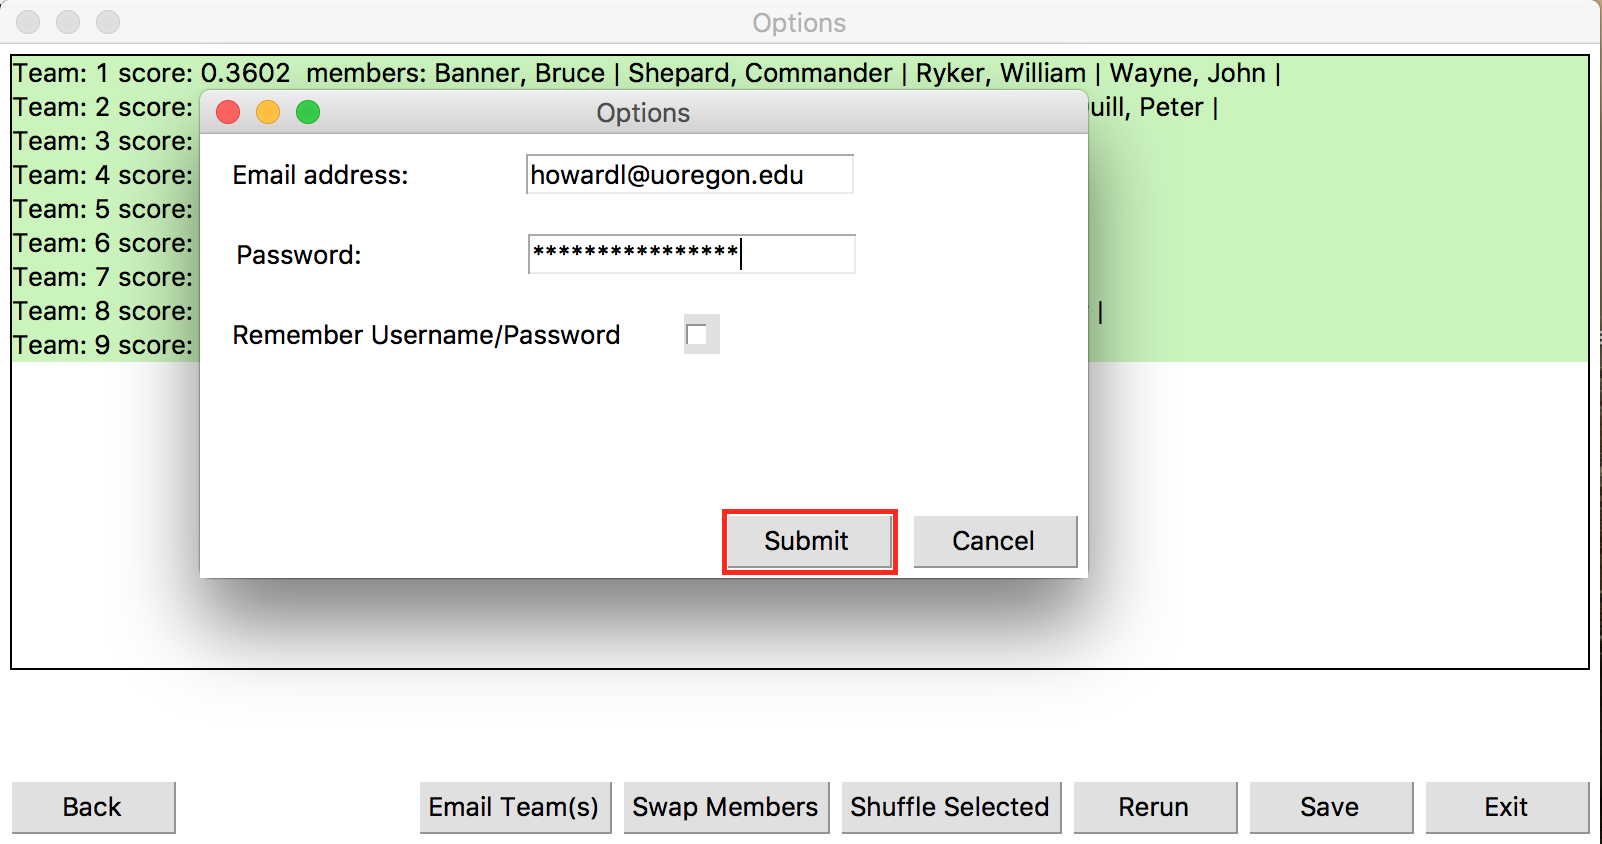
\includegraphics[width=0.6\textwidth]{pic23}
\end{figure}
\begin{figure}[h]
\caption{You should then receive a confirmation}
\centering
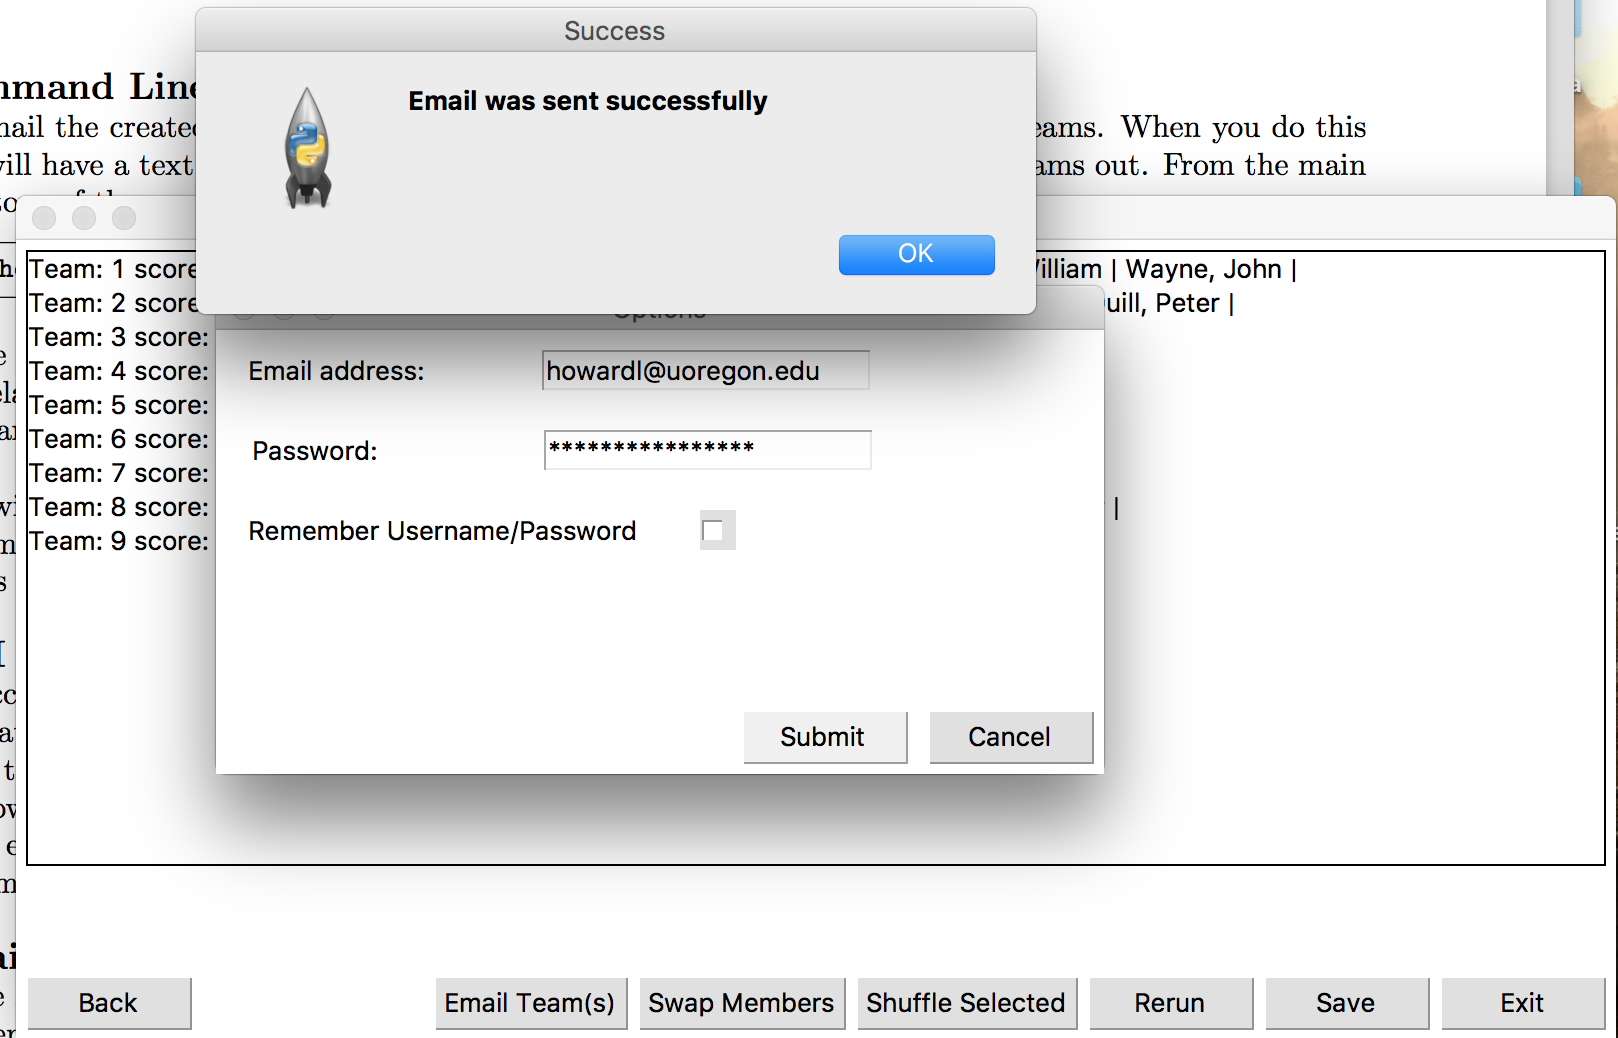
\includegraphics[width=0.6\textwidth]{pic24}
\end{figure}
The format of the email(s) is determined by the email template. Details on changing this is located below.
\\
\newline
\large
\textbf{Email Template}
\normalsize
\newline
There is an emailtemplate.txt located in to config directory. This template controls what the emails that are sent out looks like. You may change this up as you wish but it is limited currently to plain text. Instructions on what you can do to alter the template are located within the file.\\
\newline

\LARGE
Have fun team building!!!
\normalsize
\end{enumerate}
\end{document}